\documentclass{article}
\usepackage{graphicx} % Required for inserting images
\usepackage[a4paper, total={6.3in, 9.7in}]{geometry}
\usepackage{nopageno}
\usepackage{amsmath} 
\usepackage{float}
\title{Statistics in R}
\date{November 2024}


\begin{document}

\maketitle
\section{Research Question}
I chose my research question to be: How does minimum air temperature affect budburst development? My hypothesis is that there is a positive correlation between minimum air temperature and late stage budburst development.
\section{Method}
 Firstly I chose to transform the budburst data. The data contains scores from 0 to 6 for each tree, with a score of 0 representing no sign of budburst and a score of 6 representing a very high degree of budburst. Some scores included $<$ or $>$ to add detail, but I removed these for simplicity. I then transformed the scores into binomial data by splitting the scores into either success or failure data where success meant a high degree of budburst had occurred and a score of 4-6. I removed outliers that were outside of the 0-6 range as they are entry errors. This was in a data set which included a date of recording for each data point.
 
 I used a binomial generalized linear model to test whether there was a statistical significance from the minimum air temperature. I removed outliers from the minimum air temperature data that were values lower than -25 degrees celsius as there must be entry errors as they are not realistic. Since I was provided with weather data for every day across many years, I found the average minimum air temperature for the seven days preceding each budburst score data entry and this average is what I used in my generalized linear model. I did have to remove some data My response variable is therefore the binomial data for budburst score and my explanatory variable is the average minimum air temperature for the week before the budburst score was recorded. In my linear model I use the week the data is from as a fixed factor to control for changes across the season, and account for the fact that in later weeks there will be data from trees which budburst in earlier weeks, meaning the probability of trees having late stage budburst development is higher s time goes on. I created this factor by splitting the dates the scores were recorded into months and then into four groups within each month: the 1st to the 7th, 8th to the 15th, 16th to the 23rd and 24th to the 31st. In my model I used only the 6 weeks between the 8th of April to the 23rd of May as these weeks had the most data points and to simplify the model. I removed observations of budburst scores that did not have a corresponding weather data as the weather data set begins at the end of 2009, as well as data from other weeks in the year. I used data from 2010 to 2023.

 The assumption of independence of observations has been somewhat violated, there will be a relation between trees of the same species, as well each of the trees being recorded multiple times over several years, however I chose to use all the years of data and all the species I could as this increases my number of data points. This does mean that the model is less likely to be applicable to other similar trees in similar climates due to the pseudo-replication. 

I used R version 4.3.3 for the statistical analysis and the used packages dplyr, ggplot2 to filter data when transforming it and to plot Figure 1 respectivly.

\section{Results}
My model was a generalized linear model, using a binomial response variable, a continuous explanatory variable and a time as a factor. My null deviance is 105775 with 76720 degrees of freedom, and my residual deviance is 71537 with 76714 degrees of freedom, as shown in Table 1. The dispersion of this model is found using the residual deviance and corresponding degrees of freedom and is 0.93, suggesting the model is slightly under-dispersed but not very significantly. 

\begin{table} [h!]
    \caption{The null and residual deviance and degrees of freedom for the binomial generalized linear model looking at how average minimum air temperature and week affect budburst development.}
    \centering
    \begin{tabular}{|l|r|r|r|r|}
    \hline
         & Deviance & Degrees of Freedom\\
         \hline
      Null   & 105775 & 76720 \\
      Residual & 71537 & 76714 \\
      \hline
    \end{tabular}

    \label{tab:my_label}
\end{table}

This model has pseudo R$^2$ = 0.32, which is a goodness-of-fit measurement for the model as it compares the deviance of the model and compared it to the deviance of a null model. This is a fairly low pseudo R$^2$, however this is not surprising as many other factors such as tree girth may impact budburst, however I chose to just focus on minimum air temperature to simplify the model.

For every 1 degree increase in average minimum air temperature the odds of late stage budburst development increases by the e to the power of the slope, and the slope is different for each of the weeks in this time range. This is true for $\text{Odds} = \frac{\text{probability}}{1 - \text{probability}}$. This means that in week 1, for every degree increase in temperature, the odds of budburst development goes up by e$^{0.22}=1.25$ times. For week 2 the odds of budburst goes up by e$^{0.22+1.54}=5.8$. Week 3 has an odds increase of 9.11, week 4 of 18.7, week 5 of 77.5 and week 6 of 225.9. 

\begin{table}[h!]
\caption{Coefficients for the binomial generalized linear model looking at how average minimum air temperature and week affect budburst development.}
\centering
\begin{tabular}{|c|c|c|c|}
\hline
\text{Predictor} & \text{Estimate} & \text{z value} & \text{$Pr(>|z|)$} \\
\hline
Intercept          & -3.081  $\pm $        0.040           & -77.73            & $< 2 \times 10^{-16}$ \\
AvgAirMin          & 0.215   $\pm $ 0.004            & 49.81             & $< 2 \times 10^{-16}$ \\
factor(week)2      & 1.544   $\pm $ 0.041            & 37.25             & $< 2 \times 10^{-16}$ \\
factor(week)3     & 1.993   $\pm $0.041            & 49.15             & $< 2 \times 10^{-16}$ \\
factor(week)4      & 2.705   $\pm $ 0.041           & 65.66             & $< 2 \times 10^{-16}$ \\
factor(week)5     & 4.128   $\pm $0.046            & 89.17             & $< 2 \times 10^{-16}$ \\
factor(week)6     & 5.203   $\pm $ 0.064            & 81.75             & $< 2 \times 10^{-16}$ \\
\hline
\end{tabular}
\end{table}
I created a graph of the model, showing the binomial data points for the budburst development against temperature in black, with the generalized linear model shown in colour with each colour representing a different week, with error around these lines. In this graph there is a clear visual difference in the binomial data in the presence and absence of late stage budburst development. This is shown in Figure 1. 
\begin{figure}[H]
        \centering
        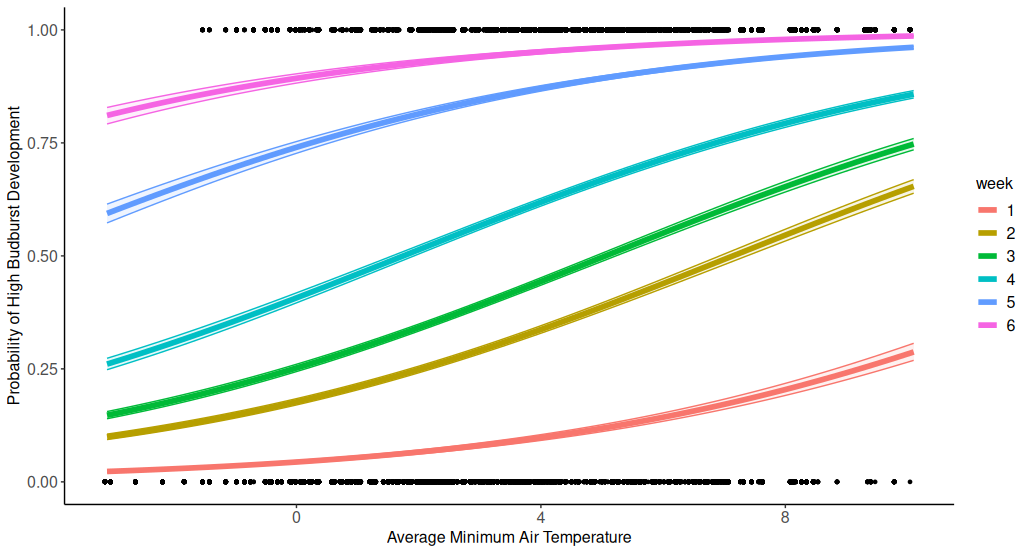
\includegraphics[width=1\linewidth]{../data/Rplot.png}
        \caption{A graph showing the binomial generalized linear model looking at how average minimum air temperature across 7-8 days affects the probability of late stage budburst development, split into weeks}
        \label{fig:enter-label}
    \end{figure}
I found the flipping point for each week, which is the average minimum air temperature for the week before a day in that week which results in half of the budbursts being at a late stage of development. This value decreases through the weeks as it is less likely that budburst will not have occurred over time. These values are shown in Table 3, and are only valid when they are within the range of the model which means between approximately -3 and 10 degrees celsius. The results in weeks 1, 5 and 6 are out of this range because the odds of late stage development in budburst is very low in week 1 and very high in week 5 and 6 due to the times of year, so having exactly half of trees in late stage budburst development is unrealistic. 

\begin{table}[h!]
    \caption{Flipping points (degrees celcius) for each week of data for the binomial generalized linear model looking at how average minimum air temperature and week affect budburst development.}
    \centering
    \begin{tabular}{|c|c|c|c|c|c|}
    \hline
        Week 1  &  Week 2  &  Week 3 &  Week 4 &  Week 5 &  Week 6\\
        \hline
        14.3 & 7.1 & 5.1 & 1.7 & -4.9 & -9.9 \\
         \hline
    \end{tabular}
\end{table}

There is a statistically significant positive relationship between average minimum air temperature and budburst development, and there is also a statistically significance in the difference in this relationship each week. This is shown as all the p values for these variables are in table 2 and they are all $<2 \times 10^{-16}$ as shown in table 2. This suggests that as average minimum air temperature increases, the probability of budburst also increases, and as time goes on the temperature needed in the last week for late stage budburst development is lower. This is because time has an influence on budburst development so in the later weeks of this study there is a higher probability of late stage budburst development at the same temperatures.



\end{document}
